\chapter{Background}

Thanks to a protective atmosphere, Earth can withstand impacts from dust to boulder-sized objects traveling faster than bullets without so much as a dent on Earth's surface.
While most of these near-Earth objects are extremely small and don't leave much of a trace, the larger objects can leave a trail of light visible from Earth's surface as they burn up in our atmosphere.
In this chapter, we will discuss the classification of near-Earth objects, how fireballs are observed, and give important insight as to why and how we will compare our photometric survey with others.


\section{Description of Fireballs}

When considering types of near-Earth objects, many names come to mind: asteroids, meteors, meteorites, and fireballs are all often used interchangeably. 
However, there are several key distinctions between these objects.  
Asteroids are the largest of this group and are generally over \SI{10}{\meter} in diameter \cite{steel_meteoroid_1996}. 
These objects are responsible for massive craters that are visibly present on the moon.
Meteoroids are anywhere between \SI{10}{\micro\meter} and \SI{10}{\meter} and are far more numerous than their asteroid cousins.  

Meteoroids that pass through Earth's atmosphere become meteors.
As a meteor passes through our atmosphere, it begins to ablate.
Ablation begins when a fast moving meteor, typically traveling over \SI{10}{\meter/\second}, encounters air particles that slow it down.
This leftover kinetic energy is turned into heat and is hot enough to vaporize outer layers of the meteor.  
Atoms within these vaporized outer layers and nearby air molecules get excited to a point where they release light.
The amount of light that reaches an observer on Earth's surface can be measured in terms of apparent magnitude.
Magnitude is represented on a $\log_{10}$ scale where dimmer objects are represented by high numbers and brighter objects are lower.
The equation for calibrated magnitude is

 $$ m = -2.5 \log_{10}(I/I_0)$$


where $I$ is the intensity of the meteor/fireball and $I_0$ is the intensity of a reference location.  
Both intensity measurements are in units of $\si{W/\meter^2}$.
Meteors with an apparent magnitude below $-4$ qualify as bolides, or fireballs.
For reference, in it's brightest phase, Venus is a magnitude $-4.4$ planet while the dimmer Jupiter has a magnitude of $-2.1$ \cite{rao_venus_nodate}.
If an object is massive enough to withstand the pressures of Earth's atmosphere and make it to the surface of Earth, it is classified as a meteorite. 
These are extremely rare, occurring less than $200$ times per year.
Because meteorites are essentially rock remnants, they provide valuable information about the initial asteroid's origins.
While there is some overlap between asteroids, meteoroids, meteors, fireballs, and meteorites, their definitions are important to distinguish.
Figure \ref{jed} summarizes the relationship between these 5 terms.

\begin{figure}[ht!]
  \centering
  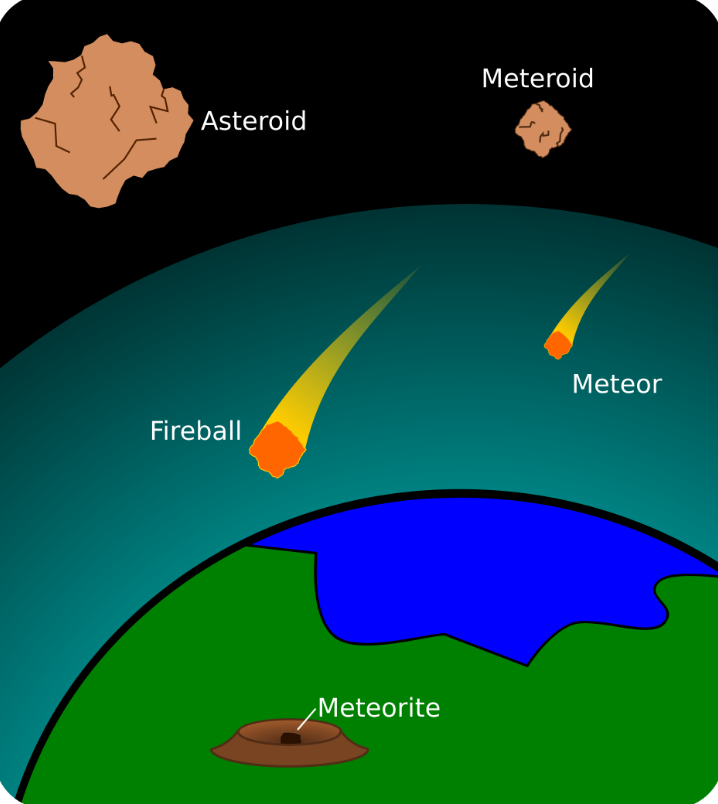
\includegraphics[scale=0.3]{images/jed_zoomedin.png}
  \caption{A depiction of near-Earth object classification.  Asteroids and meteoroids may be found in space, while meteors and their brighter counterpart, fireballs, burn up through Earth's atmosphere.  Unlike ordinary fireballs, meteorites remain intact }
  \label{jed}
\end{figure}

Our project specifically focuses on fireballs.
A fireball passing through the sky is referred to as a fireball event, and these events will provide data for our fireball catalog.
We may further classify fireball events into two categories: sporadic events and meteor shower events.
Meteor showers occur when Earth's orbit crosses paths with the orbit of a collection of debris. 
Such collections often orbit large masses such as Jupiter or the sun \cite{trigo-rodriguez_2006_2007}.  
For example, the Perseid meteor shower has a highly elliptical orbit around the sun as seen in Figure \ref{perceid}.  
As comets travel through space, small bits of rock and ice separate from them.
This process is due to differences in pressures and heat on different areas of the comet.
Comet fragments make up a majority of the substance in meteor showers.

\begin{figure}[ht!]
  \centering
  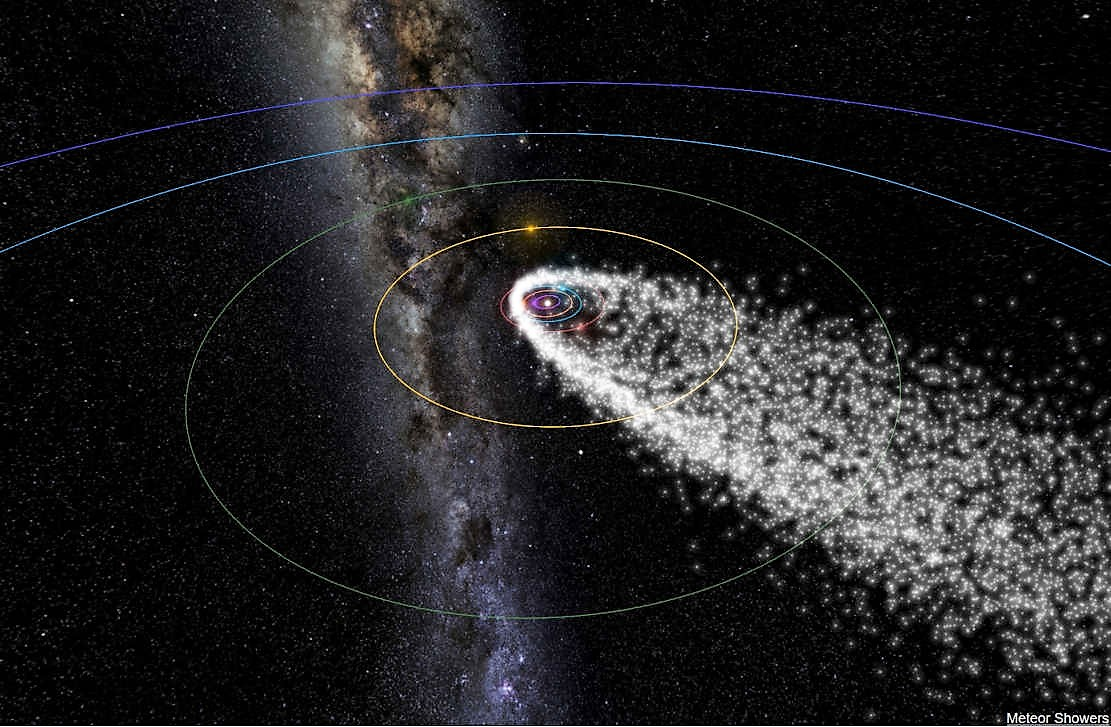
\includegraphics[scale=0.7]{images/persiod_shower.jpg}
  \caption{The Perseid meteor shower and its relation to our solar system.}
  \label{perceid}
\end{figure}

In contrast, there is debris in space that is not connected to any meteor shower. 
Events stemming from random debris are called sporadic events.
Due to the innate nature of gravity, debris in space often gets collected and becomes part of a larger system such as a meteor shower.
Thus, sporadic events are less common.
Collecting information on fireball events allows astronomy researchers to develop a better understanding of the presence of matter in space. %not super sure about this sentence but wanted some sort of transition


\section{Event Detection}

To compare our camera system to other professional systems, we must acquire enough event data to determine a flux rate.  
This section will discuss how different observation systems collect data on fireballs.
We will specifically detail how the Willamette D6 allsky camera differs from professional cameras.


\subsection{Existing Surveys}
While amateur astronomers and low-budget systems capture useful information, larger professional systems act as a vitally important comparison point.
Because many professional surveys are composed of multiple cameras working in unison, they have the advantage of multiple perspectives on a singular event.
This leads to more precise measurements of parameters like velocity, apparent magnitude, and location.
Individual events captured by an individual observer do contribute to the pursuit of knowledge.
However, a small camera system that cannot yield similar data to more professional surveys serves only a marginal amount of utility.

Cameras for allsky Meteor Surveillance (CAMS), the SPanish Meteor Network (SPMN), NASA's allsky Fireball Network and the Lincoln Near Earth Asteroid Research (LINEAR) program are examples of well-established existing meteor observing surveys.
All of these programs are continuously acquiring data and adding their findings to existing databases.  
Much of this data is widely available online, but vary from survey to survey.
% CAMS
Funded by NASA, Cameras for allsky Meteor Surveillance (CAMS) aims to verify minor meteor showers and trace them back to their existing parent comets \cite{jenniskens_cams:_2011}.  
The project was created by Peter Jenniskens and is based in California.  
The CAMS network is spread across 3 different locations as seen in Fig. \ref{trio} and consists of over 60 cameras.
Each camera is has a relatively narrow field of view $~30\deg$.
When arranged intentionally, these cameras provide a high resolution image of the entire visible sky.
By spreading their cameras across three separate locations, the CAMS research group can measure precise trajectories of incoming meteors. 

\begin{figure}[ht!]
  \centering
  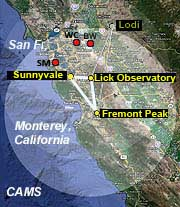
\includegraphics[scale=0.9]{images/CAMS_trio.jpg}
%   \setcaptioncitation{http://cams.seti.org/maps.html}
  \caption{The three CAMS network stations within a 50 mile radius.}
  \label{trio}
\end{figure}

Similarly to the phenomena of trying to catch a baseball with only one eye open, confidently capturing a three dimensional trajectory of a fireball is extremely difficult when using only one camera.
Multiple cameras provide different fireball-path perspectives and allow us to geometrically solve for the event's depth.
Accurate trajectories are particularly useful in back-tracing the motion of the meteor's orbit.  
The CAMS team has reduced over $320,000$ of these orbits \cite{peter_jenniskens_cameras_2018}


%SPMN
The SPanish Meteor Network (SPMN) works extremely similarly to the CAMS project.  
It consists of 25 observation stations located across Portugal and Spain \cite{trigo-rodriguez_2006_2007}.
In addition to becoming the first organization in Spain to successfully calculate the orbital path of a meteor, this organization revolutionized fireball research by developing the first CCD allsky cameras, or cameras that observe the entire visible sky. \cite{jordi_l._pique_presentation_nodate}
While this approach results in lower resolution event capturing, it is much cheaper and covers the same sky area.
These cameras are now in use all across the world.

While the SPMN and CAMS are extremely powerful research organizations, their study of meteors only slightly overlaps with the research being discussed in this paper.
Because of their high grade equipment, they are able to capture data from extremely dim sources.
Fireballs, quantified by a magnitude below $-4$, compose only a small fraction of the meteors analyzed by these organizations.
Fortunately, other organizations focus specifically on larger and brighter events.

%Peter Brown
There are a multitude of ways that one can attain information about a fireball.  
All the aforementioned surveys have employed the use of photometric data.
In contrast, Peter Brown took data from the Department of Defense and the Department of Energy space-based systems in geostationary orbits.
The original purpose of these systems is to detect signatures of explosions near Earth's surface, but the system occasionally picks up false positives in the form of ablating bolides.  
Because the systems detect the amount of power released, Brown and others have used the systems to approximate a fireball's energy.
In a 2002 article published by \textit{Nature}, Brown estimated the optical energies of around 300 bolides.
Drawing from this data set and other existing data sets, Brown created compiled the following equation which relates bolide energy to the number of impacts on Earth each year. 

\begin{equation}
\log N = a_0 - b_0\log E
\label{eq:browneq}
\end{equation}
where $N$ is the total number of objects colliding with earth each year and $E$ is the respective energy of the sample in kilotons \cite{brown_p_flux_2002}.
In this empirically derived equation, $a_0 = 0.5677 \pm 0.015$ while $b_0 = 0.90 \pm 0.03$.
This relationship is known as a power law and will be useful to compare our Willamette D6 allsky data with.


%%%%%%%%%%%%%%%%%%%%%%%


\subsection{The D6 Allsky Camera}

% Overview
The Willamette University D6 allsky camera was created in 2016 to capture images of fireballs streaking through the night sky.
The aim of the project was to create an economically feasible and highly mobile observational system.
The Willamette D6 allsky camera was constructed by Kyle McSwain alongside Dr.\ Jed Rembold in 2006.
It is composed of a portable structure surrounding a state-of-the-art camera system along with necessary supporting devices, including a controlling Raspberry Pi. \cite{mcswain_using_2016}.
The assembly resembles a Star Wars astromech droid, and acquired its name from this inspiration.
The enclosure with visible camera is shown in Fig. \ref{droid}.
The D6 allsky camera is currently operational and has been gathering data since the summer of 2018.  
Below, we will discuss the design of the D6 allsky camera while also highlighting what makes it significant.

\begin{figure}[ht!]
  \centering
  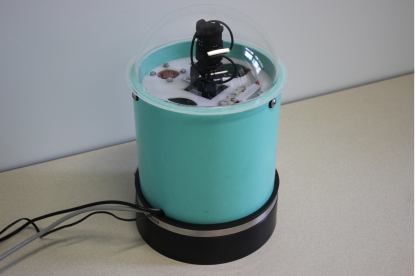
\includegraphics[scale=0.7]{images/allsky_camera.png}
  \caption{The Willamette D6 allsky camera (2016). Paired with a little imagination it resembles an astromech droid from Star Wars.\inlinecomment{We should get a new image of this, as it has the sealing cowl along the top now.}}
  \label{droid}
\end{figure}


% Components
The components of the D6 allsky camera are comprised primarily of 5 different pieces: the camera housing, a CCD camera, a thermostat, a digitizer, and the Raspberry Pi to control everything.
The acrylic dome and PVC shell form the exterior of our system. 
The dome itself is a transparent half sphere that sits on top of a PVC cylinder that holds the system together.
Both act as a protective layer between the sensitive inside components and the outside environment.  
Without this feature, the system would be subject to rain, snow, dew, bug contamination, and other undesired effects.

The CCD camera is perhaps the most important feature of the system.
The Watec $902$H$2$ CCD camera uses a fish-eye lens to observe the entire visible night sky.
It was chosen due to its extremely high sensitivity and resolution \cite{noauthor_wat-902h2_nodate}.
However, it should be noted that more expensive systems consisting of multiple cameras (like CAMS) provide an even higher resolution of fireball events.

Because of its constant use throughout the night, the system itself can get very warm and therefore needs some thermal regulation.
The inside components are kept at a relatively constant temperature above the dew point by a thermostat and a fan system.
The camera outputs an analog signal which requires the use of a digitizer before it can be processed by the Raspberry Pi.
The coaxial signal is sent to the digitizer before connecting to the Raspberry Pi via USB.

% Uniqueness
While there are several similarities in the composition of our allsky camera to existing systems, there are several key differences.
The most prominent of these are the size, versatility, and cost of our system.
Around the size of a basketball, the D6 allsky camera is extremely compact.  
Not only is it small, but it only relies on a single power chord for power.  
Because of this, the camera can be easily picked up and relocated to any setting that has a power source.  
The system has low power requirements and it should be possible to run from a battery if remote placement is desirable in the future.
Other systems, such as several CAMS camera setups are rooted to extremely powerful computers that have little to no mobility as shown in Fig. \ref{immobile}.

\begin{figure}[ht!]
  \centering
  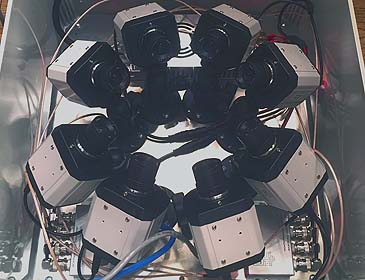
\includegraphics[scale=0.7]{images/Florida-CAMSbox-thumb.jpg}
  \caption{An entrenched alternative fireball observation system.}
  \label{immobile}
\end{figure}

This presents issues related to being rooted in one location such as building renovation or sporadic light pollution issues.
For example, if a tree were to grow near the camera, it would need to be chopped down or the entire system may need to be relocated.
With the lightweight and portable D6 allsky camera, relocation is not a difficult process.

Additionally, the D6 allsky camera is a less expensive alternative to other fireball analysis tools.
The ingenuity of running initial analysis on a microcomputer allows the D6 allsky camera to cost a fraction of what professional systems cost.
Although large professional organizations produce copious amounts of wonderful data, in the field of fireball research, amateur systems outnumber professional systems $2:1$ \cite{gural_review_2005}. 
Providing a cost efficient alternative could be a great way to expand the field of fireball research and in turn provide a better understanding of the near-Earth objects in our solar system.


\section{Photometry}
After collecting videos of potential fireballs, next comes the task of analyzing the videos.
Luke Russell, advised by Dr. Jed Rembold, wrote a photometry program in Python that allows us to get a calibrated light curve for a given video of a fireball.
Simply running a fireball video through his interactive GUI allows us to access information about luminous properties of the fireball.
However, limitations to our photometry must be taken into account.
False positives, extinction, and other error factors must be accounted and corrected for while creating our fireball catalog.

\subsection{Existing photometry tools}
The primary photometric analysis tool that we use is a Photometry GUI in which a user interacts with a fireball video.
After selecting both of these and entering in the known magnitude of the reference star, our photometry program automatically tracks the fireball throughout the following frames.
By using Gaussian fits to the photometric data, the program is able to center its view on the fireball and determine its size throughout its path.
Throughout this process, the video also sums the photon counts for each fireball pixel for each frame.
This photon count gives us the magnitude of the fireball at a given point in its path.
Doing this for each frame results in a light curve that shows the magnitude as a function of time, which yields the valuable light curve.
From this light curve, we can then move on to further analysis.

\subsection{False Positives and Atmospheric Extinction}

While it is able to capture fireballs, the D6 allsky camera still picks up a great deal of false positives.
In an initial sample of over $700$ videos, only $2$ of them contained real events.
The vast majority of the videos were of bugs crawling across the acrylic dome.
Because the bugs are illuminated by nearby light, they appear to be bright spots traveling across the screen and thus the detection script mistakenly flags them as fireball events.
Moreover, many bugs are featured in several videos as they have a tendency to move, stop somewhere, and move again.
While this is somewhat problematic, we aim to implement several steps to limit the number of false positive bug cases.
We aim to implement video length restrictions, and linear motion restrictions to limit the number of false positives.

In addition to bugs, other events such as airplanes, satellites, and Iridium flares provide false-positive videos.
Their near-linear motion and bright presence are an instant trigger for the fireball detection.
A larger problem in data analysis stems from the phenomena of atmospheric extinction.
As shown in Figure \ref{extinc}, we observe that when looking close to the horizon, light must travel through a larger volume of atmosphere than it does for an observation close to the zenith.  
Because the light travels through more atmosphere, more of the light is absorbed by gases or scattered by air particulates \cite{hughes_atmospheric_2016}.


\begin{figure}[ht!]
  \centering
  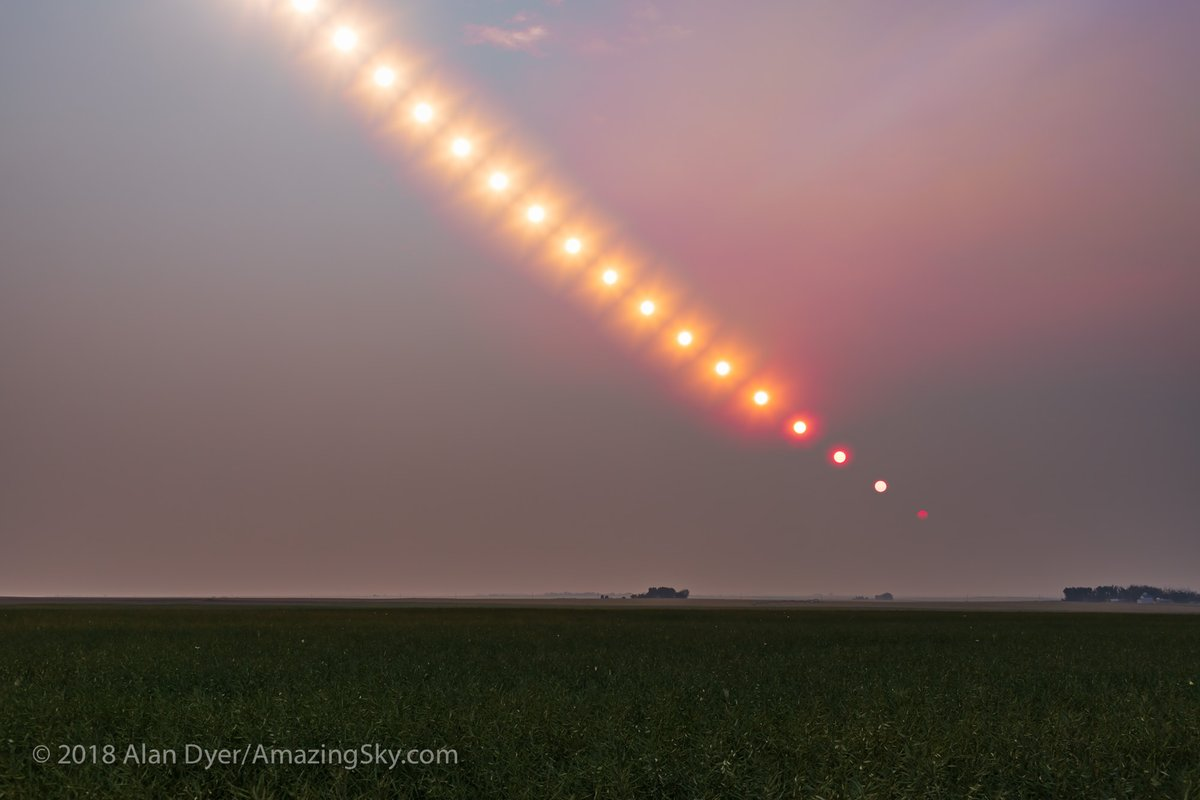
\includegraphics[scale=0.25]{images/sunset.jpg}
  \caption{A depiction of atmospheric extinction's effect on a sunset on a smokey day.}
  \label{extinc}
\end{figure}


Part of this project will include accounting for atmospheric extinction in a secondary photometric analysis script.
This will involve measuring the light intensity of known reference stars at various pixel locations throughout the night and comparing them to the real intensity values.
This will allow us to have calibration values for different pixel locations throughout our camera's frames, and thus will be applicable to any event's analysis.


\section{Parameters of Interest}

As previously mentioned, the most critical component of our analysis is the final measured flux of our system. 
To recreate a plot similar to Fig. \ref{brown}, we must have multiple events, estimated energies/masses of each event, total area of sky covered, and the total observation time.
This section will detail how we will go about collecting this information.


\subsection{Fireball Mass and Energy}

Because of the limitations of using one camera system, we will make several key assumptions in determining any fireball's initial mass and energy.  
Firstly, we assume the velocity of the fireball.
This will vary depending on the associated meteor shower.
Additionally, we will assume a luminous efficiency, $\tau$, on a similar basis.
The following equation can be used to determine the optical energy of a fireball.
$$
\tau = (0.1212 \pm 0.0043)E_0^{0.115 \pm 0.075}
$$
Optical energy is useful, as it proved us a relationship to total fireball energy through the following equation.
$$ E = 8.2508(E_0)^0.885$$
This is an empirically derived formula based on data taken by Peter Brown \cite{brown_p_flux_2002}.  
Now that we have a clear image of how to determine energy, we can transition to finding the initial mass of a given event.
To do this, we will need the mass and radius of the fireball.

Paired with our assumption that fireballs on average have a density of \rule{1cm}{.1pt} and a generally spherical shape, we can calculate the diameter using the following equation,

$$d = 2(\frac{3m}{4\pi \rho})^{1/3}$$
where $\rho$ represents the density of the fireball prior to entering the atmosphere.
%%%%%%%%%%%%%%%%%%%%%%%%%%%%%%%%%%%%
% I can't seem to find your dissertation online...
% Also, how do I account for it changing in time???
% Also why is there a $m$ in the diameter equation???
%%%%%%%%%%%%%%%%%%%%%%%%%%%%%%%%%%%%
\comment{I will definately still need help in this section}


The light curve outputted by our existing photometry GUI allows gives us light intensity at any given time.
The luminosity is then related to the intensity of the fireball through the following formula,
$$ I = \frac{L}{4 \pi r^2}$$
where $I$ is the intensity, $L$ is the luminosity, and $r$ is the radius of the object in question.  
The radius is easily attainable from the diameter.
This luminosity will help us estimate the initial mass of the object in question.
Equation \ref{eq:mass} can be used to determine the initial mass of an ablating meteor,
\begin{equation}
m = \int \frac{2L}{\tau v^2} dt
\label{eq:mass}
\end{equation}
where $L$ is the luminosity, $dt$ is the change in time, $v$ is velocity, and $tau$ is the luminous efficiency. 


\subsection{Time Observed}

Each individual video or night snapshot taken by the Willamette D6 allsky camera is labeled with a time stamp.  
In addition to this useful time documentation, when operating, our allsky camera has a running log of its functions.
This well-kept documentation allows us to keep track of the total observation time, a critical component of determining flux.  
However, there are certain limitations associated with the amount of time we can observe.

Primarily taking data in Salem, Oregon, the Willamette D6 allsky camera is subject to weather in the pacific northwest.  
Rain and cloudy nights limit the number of days we may take data.
Luckily, the versatility of the camera system allows for it to be taken to alternative locations during school breaks or periods of bad weather.


\subsection{Total Observation Area}
One factor that is particularly difficult to deal with when considering flux is the area of the sky that is being observed at a given time.
Using basic trigonometry, we can work out that:

\begin{equation}
    \text{Sky Coverage} = \Omega(h+r)^2
    \label{area_eq}
\end{equation}

where $\Omega$ is the steradian, or solid angle from earth, $h$ is the height above Earth's surface, and $r$ is the radius of Earth.
We will get a concrete steradian value by comparing angular distance to pixel distance in our camera frames.
To expand on this, when a moon travels through the night's sky, it covers a angular distance in the sky.  
If it were to travel from one horizon directly through the zenith to the other horizon, it would have traveled an angular distance of $180 \deg$.  
If we know the angular distance traveled and the total number of pixels traversed, we can establish a relationship between the two and get a precise steradian value.
Plugging this value into Eq. \ref{area_eq} yields a sky coverage area.

One might naively assume that the total observation area would remain consistent each night.
However, one must consider clouds and fog when calculating the overall sky area covered.
This consideration will be dealt with in our secondary analysis and is further discussed in the methods section.
